\documentclass{article}

\usepackage{fontspec}
\usepackage{fullpage}
\usepackage{multicol}
\usepackage{multirow}
\usepackage{tikz}

\begin{document}

\newfontfamily\swfill{SuttonSignWritingFill.ttf}
\newfontfamily\swline{SuttonSignWritingLine.ttf}
\newcommand{\bul}{\hfil$\bullet$&}
\renewenvironment{glossary}{\begin{multicols}{5}\begin{center}}{\end{center}\end{multicols}}
\setcounter{secnumdepth}{0}
\setlength{\columnseprule}{1pt}

\section{Supplement For Lesson 10}

\begin{center}
\it
Objectives inspired by, vocabulary transcribed from, and sentences and story by Bill Vicars.

Handshape photos by Adam Frost.

No endorsement implied nor given by either.
\end{center}

\subsection{Objectives}

\begin{tabular}{p{1cm}p{14cm}}
\bul I have completed the objectives for this lesson.\\
\bul I know which base symbols are in Symbol Groups curve floor and circle.\\
\bul I am able to read, write, and sign half of the ASL handshapes in symbol group six.\\
\bul I am able to recognize the vocabulary for this lesson.\\
\bul I am able to read the practice sentences for this lesson.\\
\bul I am able to read the practice story for this lesson.\\
\end{tabular}

\subsection{Symbol Groups Curve Floor and Circle}

The nineteenth Symbol Group we informally call curve floor, though its official name is ``Curves Parallel Floor Plane''.

\begin{center}
\begin{tabular}{rcrc}
\textbf{Base Symbol}&\textbf{Example}&\textbf{Base Symbol}&\textbf{Example}\\
Curve Floor Plane Small         &B511x505S2d500489x496&Curve Floor Plane Medium 1 &B515x506S2d600486x494\\
Curve Floor Plane Medium 2      &B520x507S2d700481x493&Curve Floor Plane Large    &B523x508S2d800477x493\\
Curve Floor Plane Combined      &B519x510S2d900481x490&Hump Floor Plane Small     &B520x506S2da00480x495\\
Loop Floor Plane Small          &B520x506S2db00480x495&Wave Floor Plane Snake     &B525x507S2dc00476x494\\
Wave Floor Plane Small          &B521x508S2dd00479x492&Wave Floor Plane Large     &B525x511S2de00475x490\\
Rotation Single Floor Plane     &B511x511S2df00490x490&Rotation Double Floor Plane&B511x515S2e000490x486\\
Rotation Alternating Floor Plane&B512x515S2e100489x486&Shaking Parallel Floor     &B510x516S2e200490x484\\
\end{tabular}
\end{center}

The twentieth Symbol Group we informally call circle, though it's official name is ``Circles''.

\begin{center}
\begin{tabular}{rcrc}
\textbf{Base Symbol}&\textbf{Example}&\textbf{Base Symbol}&\textbf{Example}\\
Arm Circle Wall Small Single      &B512x514S2e300489x487&Arm Circle Wall Medium Single     &B515x517S2e400486x484\\
Arm Circle Wall Small Double      &B512x514S2e500489x487&Arm Circle Wall Medium Double     &B515x517S2e600486x484\\
Arm Circle Hits Wall Small Single &B508x513S2e700493x488&Arm Circle Hits Wall Medium Single&B507x516S2e800493x484\\
Arm Circle Hits Wall Large Single &B507x520S2e900493x480&Arm Circle Hits Wall Small Double &B508x513S2ea00493x488\\
Arm Circle Hits Wall Medium Double&B508x516S2eb00493x484&Arm Circle Hits Wall Large Double &B507x520S2ec00493x480\\
Wrist Circle Front Wall Single    &B509x512S2ed00492x489&Wrist Circle Front Wall Double    &B511x512S2ee00490x489\\
Wrist Circle Hits Wall Single     &B509x510S2ef00491x490&Wrist Circle Hits Wall Double     &B511x510S2f000490x490\\
Finger Circles Wall Single        &B508x509S2f100492x492&Finger Circles Wall Double        &B508x509S2f200492x492\\
Finger Circles Hits Wall Single   &B505x511S2f300496x489&Finger Circles Hits Wall Double   &B505x511S2f400495x489\\
Arrowheads Small                  &B507x504S2f500494x497&Arrowheads Large                  &B508x504S2f600492x496\\
\end{tabular}
\end{center}

Before you can consider this lesson complete, you need to be able to list off the symbol grops as:
``one, two, three, four, five, six, seven, eight, nine, thumb;''
``contact, finger, wall, diagonal, floor, curve wall, hit wall, hit floor, curve floor, circle.''

Final help for the second set of base symbols.
All of our informal names are in the singular even if it might make more sense to have plural --- so we use eye instead of eyes.

\subsection{First ASL Handshapes From Symbol Group Six}

The eleven handshapes in Symbol Group Six used by ASL in order are:
{\bf
Index Middle Ring;
Index Middle Ring on Circle;
Index Middle Ring, Bent;
Index Middle Ring, Unit;
Index Middle Ring, Unit Hinge;
Baby Up;
}
Baby Thumb;
Baby Thumb on Hinge;
Baby Index Thumb;
Baby Index Thumb on Hinge;
and Baby Index.

\subsubsection{The Index Middle Ring Handshape}

\begin{center}
\begin{tabular}{r*{6}{c}}
&\textbf{Fill 1}&\textbf{Fill 2}&\textbf{Fill 3}&\textbf{Fill 4}&\textbf{Fill 5}&\textbf{Fill 6}\\
\multirow{2}{*}{\textbf{Right}}&
B509x515S18600491x485&
B509x515S18610491x485&
B509x515S18620491x485&
B509x515S18630491x485&
B509x515S18640491x485&
B509x515S18650491x485\\
&
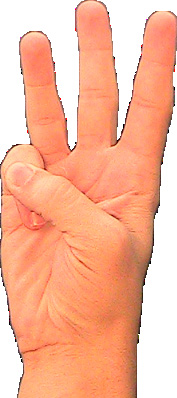
\includegraphics[scale=0.1]{images/06-01-1.jpg}&
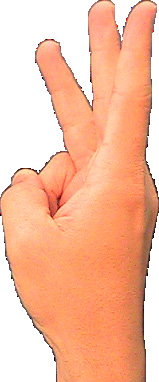
\includegraphics[scale=0.1]{images/06-01-2.jpg}&
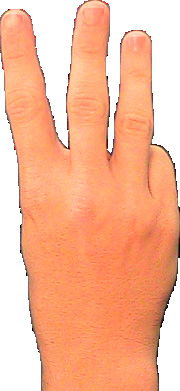
\includegraphics[scale=0.1]{images/06-01-3.jpg}&
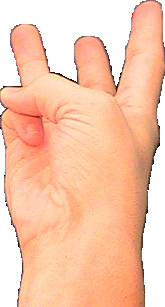
\includegraphics[scale=0.1]{images/06-01-4.jpg}&
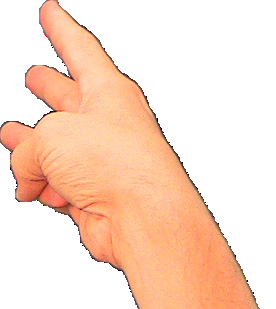
\includegraphics[scale=0.1]{images/06-01-5.jpg}&
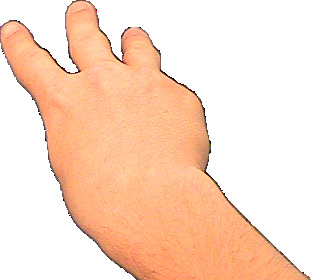
\includegraphics[scale=0.1]{images/06-01-6.jpg}\\
\textbf{Left}&
B509x515S18608491x485&
B509x515S18618491x485&
B509x515S18628491x485&
B509x515S18638491x485&
B509x515S18648491x485&
B509x515S18658491x485\\
\end{tabular}
\end{center}

\subsubsection{The Index Middle Ring On Circle Handshape}

\begin{center}
\begin{tabular}{r*{6}{c}}
&\textbf{Fill 1}&\textbf{Fill 2}&\textbf{Fill 3}&\textbf{Fill 4}&\textbf{Fill 5}&\textbf{Fill 6}\\
\multirow{2}{*}{\textbf{Right}}&
B509x515S18700491x486&
B509x515S18710491x486&
B509x515S18720491x486&
B509x515S18730491x486&
B509x515S18740491x486&
B509x515S18750491x486\\
&
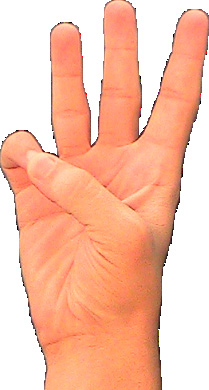
\includegraphics[scale=0.1]{images/06-02-1.jpg}&
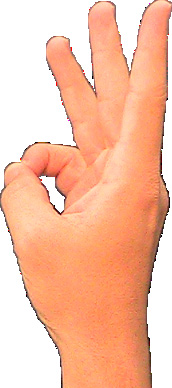
\includegraphics[scale=0.1]{images/06-02-2.jpg}&
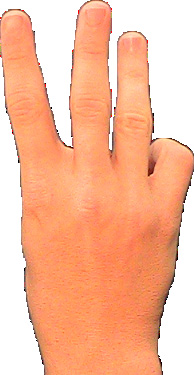
\includegraphics[scale=0.1]{images/06-02-3.jpg}&
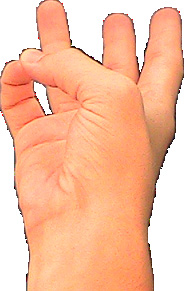
\includegraphics[scale=0.1]{images/06-02-4.jpg}&
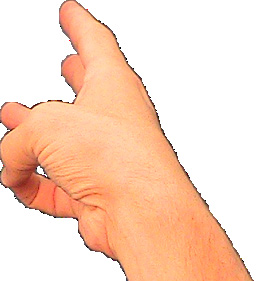
\includegraphics[scale=0.1]{images/06-02-5.jpg}&
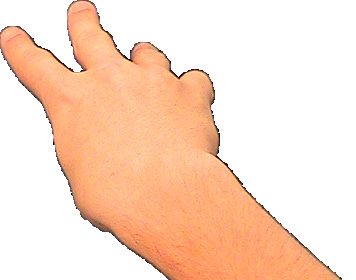
\includegraphics[scale=0.1]{images/06-02-6.jpg}\\
\textbf{Left}&
B509x515S18708491x486&
B509x515S18718491x486&
B509x515S18728491x486&
B509x515S18738491x486&
B509x515S18748491x486&
B509x515S18758491x486\\
\end{tabular}
\end{center}

\subsubsection{The Index Middle Ring, Bent Handshape}

\begin{center}
\begin{tabular}{r*{6}{c}}
&\textbf{Fill 1}&\textbf{Fill 2}&\textbf{Fill 3}&\textbf{Fill 4}&\textbf{Fill 5}&\textbf{Fill 6}\\
\multirow{2}{*}{\textbf{Right}}&
B510x515S18b00490x485&
B510x515S18b10490x485&
B510x515S18b20490x485&
B510x515S18b30490x485&
B510x515S18b40490x485&
B510x515S18b50490x485\\
&
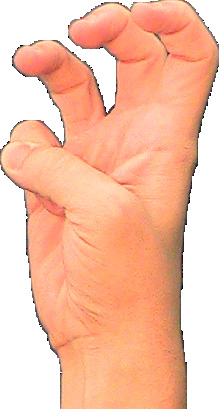
\includegraphics[scale=0.1]{images/06-03-1.jpg}&
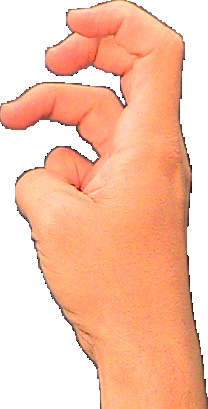
\includegraphics[scale=0.1]{images/06-03-2.jpg}&
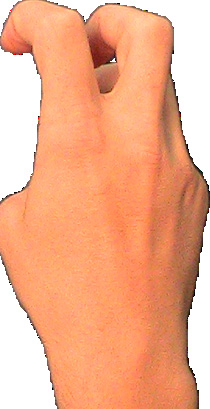
\includegraphics[scale=0.1]{images/06-03-3.jpg}&
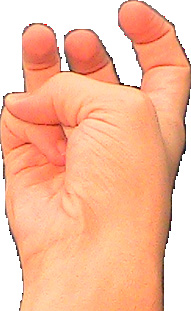
\includegraphics[scale=0.1]{images/06-03-4.jpg}&
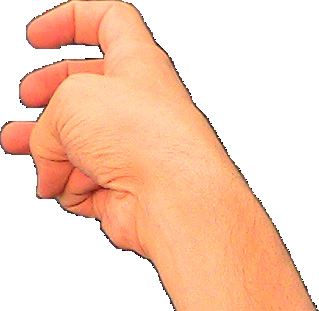
\includegraphics[scale=0.1]{images/06-03-5.jpg}&
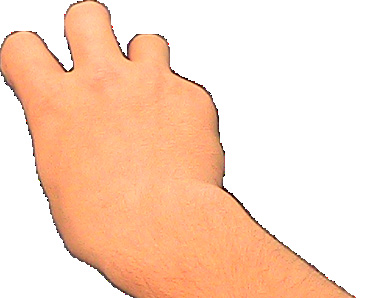
\includegraphics[scale=0.1]{images/06-03-6.jpg}\\
\textbf{Left}&
B510x515S18b08490x485&
B510x515S18b18490x485&
B510x515S18b28490x485&
B510x515S18b38490x485&
B510x515S18b48490x485&
B510x515S18b58490x485\\
\end{tabular}
\end{center}

\subsubsection{The Index Middle Ring, Unit Handshape}

\begin{center}
\begin{tabular}{r*{6}{c}}
&\textbf{Fill 1}&\textbf{Fill 2}&\textbf{Fill 3}&\textbf{Fill 4}&\textbf{Fill 5}&\textbf{Fill 6}\\
\multirow{2}{*}{\textbf{Right}}&
B508x515S18c00493x485&
B508x515S18c10493x485&
B508x515S18c20493x485&
B508x515S18c30493x485&
B508x515S18c40493x485&
B508x515S18c50493x485\\
&
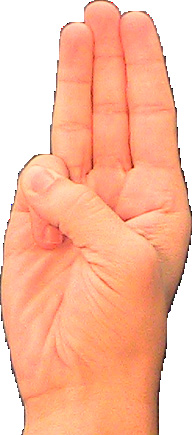
\includegraphics[scale=0.1]{images/06-04-1.jpg}&
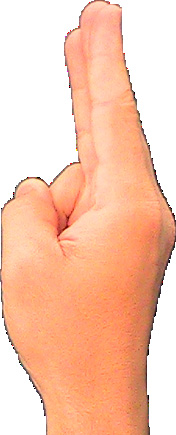
\includegraphics[scale=0.1]{images/06-04-2.jpg}&
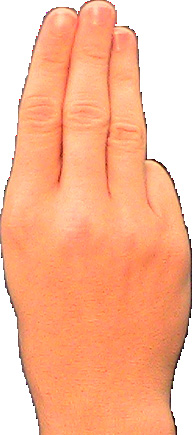
\includegraphics[scale=0.1]{images/06-04-3.jpg}&
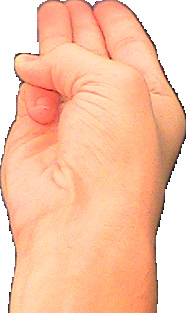
\includegraphics[scale=0.1]{images/06-04-4.jpg}&
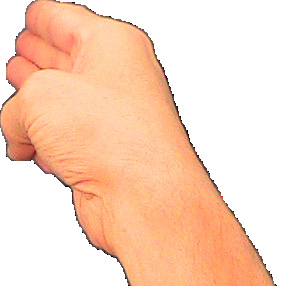
\includegraphics[scale=0.1]{images/06-04-5.jpg}&
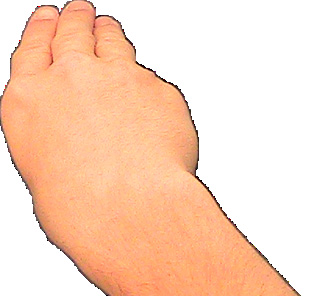
\includegraphics[scale=0.1]{images/06-04-6.jpg}\\
\textbf{Left}&
B508x515S18c08493x485&
B508x515S18c18493x485&
B508x515S18c28493x485&
B508x515S18c38493x485&
B508x515S18c48493x485&
B508x515S18c58493x485\\
\end{tabular}
\end{center}

\subsubsection{The Index Middle Ring, Unit Hinge Handshape}

\begin{center}
\begin{tabular}{r*{6}{c}}
&\textbf{Fill 1}&\textbf{Fill 2}&\textbf{Fill 3}&\textbf{Fill 4}&\textbf{Fill 5}&\textbf{Fill 6}\\
\multirow{2}{*}{\textbf{Right}}&
B510x513S18d00490x488&
B510x513S18d10490x488&
B510x513S18d20490x488&
B510x513S18d30490x488&
B510x513S18d40490x488&
B510x513S18d50490x488\\
&
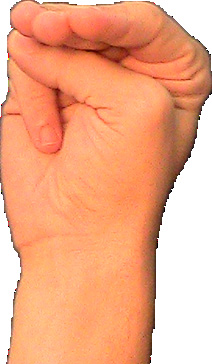
\includegraphics[scale=0.1]{images/06-05-1.jpg}&
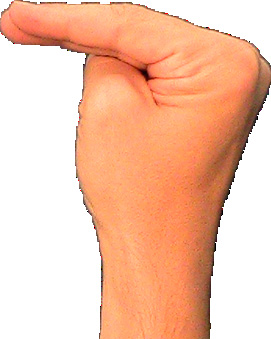
\includegraphics[scale=0.1]{images/06-05-2.jpg}&
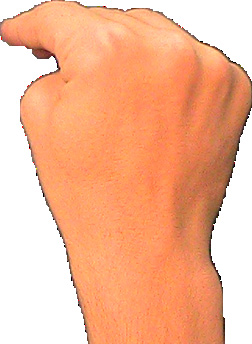
\includegraphics[scale=0.1]{images/06-05-3.jpg}&
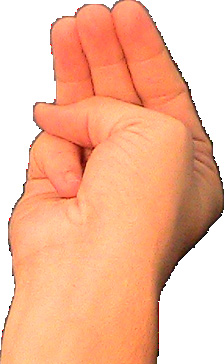
\includegraphics[scale=0.1]{images/06-05-4.jpg}&
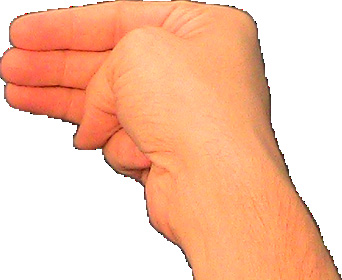
\includegraphics[scale=0.1]{images/06-05-5.jpg}&
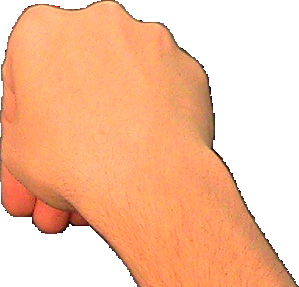
\includegraphics[scale=0.1]{images/06-05-6.jpg}\\
\textbf{Left}&
B510x513S18d08490x488&
B510x513S18d18490x488&
B510x513S18d28490x488&
B510x513S18d38490x488&
B510x513S18d48490x488&
B510x513S18d58490x488\\
\end{tabular}
\end{center}

\subsubsection{The Baby Up Handshape}

\begin{center}
\begin{tabular}{r*{6}{c}}
&\textbf{Fill 1}&\textbf{Fill 2}&\textbf{Fill 3}&\textbf{Fill 4}&\textbf{Fill 5}&\textbf{Fill 6}\\
\multirow{2}{*}{\textbf{Right}}&
B511x510S19200490x491&
B511x510S19210490x491&
B511x510S19220490x491&
B511x510S19230490x491&
B511x510S19240490x491&
B511x510S19250490x491\\
&
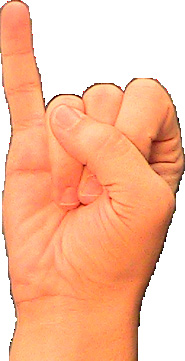
\includegraphics[scale=0.1]{images/06-06-1.jpg}&
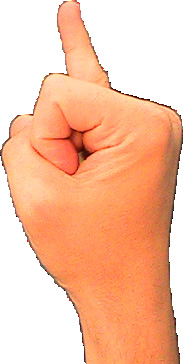
\includegraphics[scale=0.1]{images/06-06-2.jpg}&
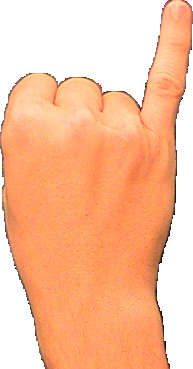
\includegraphics[scale=0.1]{images/06-06-3.jpg}&
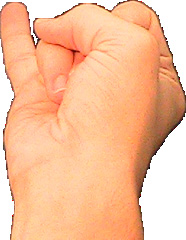
\includegraphics[scale=0.1]{images/06-06-4.jpg}&
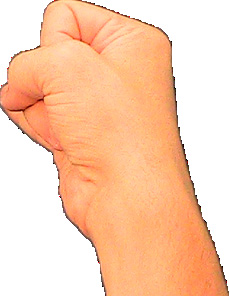
\includegraphics[scale=0.1]{images/06-06-5.jpg}&
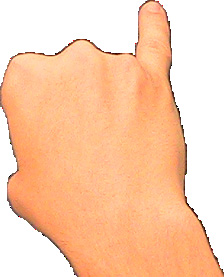
\includegraphics[scale=0.1]{images/06-06-6.jpg}\\
\textbf{Left}&
B511x510S19208490x491&
B511x510S19218490x491&
B511x510S19228490x491&
B511x510S19238490x491&
B511x510S19248490x491&
B511x510S19258490x491\\
\end{tabular}
\end{center}

\subsection{Vocabulary}

\begin{glossary}

\textbf{adopt}\\
AS14c50S14c58S22a00S22a10S20350S20358S2fb00M532x534S14c50508x503S20358472x466S20350512x466S22a00513x484S14c58468x503S22a10473x484S2fb00492x485

\textbf{bird}\\
AS1f420S22114S2ff00M518x528S2ff00482x483S1f420479x513S22114454x506

\textbf{book}\\
AS15a10S15a18S2e004S2e01cM523x529S15a10502x472S15a18486x472S2e01c477x501S2e004502x501

\textbf{bug}\\
AS12110S21800S33200M518x518S33200482x483S12110464x484S21800463x474

\textbf{cat}\\
AS1d410S20e00S26a06S2ff00M556x525S2ff00482x483S20e00513x512S26a06542x498S1d410515x487

\textbf{cow}\\
AS19a10S2df04S2ff00M544x530S2ff00482x483S19a10516x484S2df04521x509

\textbf{dog}\\
AS13810S20e00S22a04S1f000M515x534S13810489x466S20e00485x490S1f000486x519S22a04501x499

\textbf{evaporate}\\
AS14c50S14c58S22a00S22a10S20350S20358S2fb00M532x534S14c50508x503S20358472x466S20350512x466S22a00513x484S14c58468x503S22a10473x484S2fb00492x485

\textbf{fish}\\
AS15d48S2dc06M510x543S15d40491x516S2dc06494x458

\textbf{get}\\
AS14c10S14c18S26524S20340S20348S21600S21600M523x548S20340492x516S20348491x533S26524493x495S21600510x537S21600480x519S14c10500x452S14c18478x464

\textbf{horse}\\
AS13220S22114S2ff00M537x518S2ff00482x483S13220514x468S22114508x459

\textbf{indeed}\\
AS10010S26500S33b00M534x541S33b00482x483S10010487x511S26500520x497

\textbf{know}\\
AS15a11S20600S2ff00M539x518S2ff00482x483S15a11516x481S20600501x467

\textbf{look like}\\
AS19c10S19a20S20500S27106S2ff00M534x607S2ff00482x483S20500500x497S19c10490x508S19a20506x543S27106512x567

\textbf{pet}\\
AS15a51S15a57S20e00S22120M532x520S15a57469x481S15a51487x497S22120510x494S20e00498x485

\textbf{read}\\
AS10e41S15a07S22b03M524x525S10e41499x481S15a07477x475S22b03479x501

\textbf{real}\\
AS10010S26500S33b00M534x541S33b00482x483S10010487x511S26500520x497

\textbf{same}\\
AS19a20S27106M514x533S19a20486x468S27106495x493

\textbf{some}\\
AS15d41S15a36S21100S26505M527x517S15a36477x501S15d41473x483S21100502x488S26505514x504

\textbf{sure}\\
AS10010S26500S33b00M534x541S33b00482x483S10010487x511S26500520x497

\textbf{take}\\
AS14c50S14c58S22a00S22a10S20350S20358S2fb00M532x534S14c50508x503S20358472x466S20350512x466S22a00513x484S14c58468x503S22a10473x484S2fb00492x485

\textbf{take up}\\
AS14c50S14c58S22a00S22a10S20350S20358S2fb00M532x534S14c50508x503S20358472x466S20350512x466S22a00513x484S14c58468x503S22a10473x484S2fb00492x485

\textbf{tell}\\
AS10000S20500S26600S33b00M536x542S33b00482x483S20500508x516S26600520x504S10000488x512

\textbf{time}\\
AS10013S15a1aS20500M521x518S10013490x482S15a1a494x506S20500480x505

\textbf{true}\\
AS10010S26500S33b00M534x541S33b00482x483S10010487x511S26500520x497

\end{glossary}

\subsection{Practice Sheet 10.A}

\begin{multicols}{5}
\begin{center}

M508x515S10000493x485 % 1
M536x504S38800464x496 % .
M518x518S30a00482x483 % y/n
M556x525S2ff00482x483S20e00513x512S26a06542x498S1d410515x487 % cat
M516x540S1bb02488x461S14c02484x517S20e00499x502S26500499x483 % like
M528x537S33b00482x483S18507502x510S20500518x509 % eat
M518x528S2ff00482x483S1f420479x513S22114454x506 % bird
M536x507S38900464x493 % ?
\vfil
\columnbreak

M508x515S10e00493x485 % 2
M536x504S38800464x496 % .
M523x529S15a10502x472S15a18486x472S2e01c477x501S2e004502x501 % book
M510x523S10040495x493S26500491x478 % you
M516x540S1bb02488x461S14c02484x517S20e00499x502S26500499x483 % like
M524x525S10e41499x481S15a07477x475S22b03479x501 % read
M537x504S38700463x496 % ,
M518x518S30c00482x483 % \?
M524x532S14249491x508S14240477x480S2e800510x469S20500480x509 % kind
M536x507S38900464x493 % ?
\vfil
\columnbreak

M512x515S11e00489x485 % 3
M536x504S38800464x496 % .
M518x518S30a00482x483 % y/n
M510x543S15d40491x516S2dc06494x458 % fish
M516x540S1bb02488x461S14c02484x517S20e00499x502S26500499x483 % like
M528x537S33b00482x483S18507502x510S20500518x509 % eat
M518x518S33200482x483S12110464x484S21800463x474 % bug
M536x507S38900464x493 % ?
\vfil
\columnbreak

M511x516S14400489x485 % 4
M536x504S38800464x496 % .
M515x511S21802485x493S16d40497x490 % milk
M537x504S38700463x496 % ,
M518x518S30c00482x483 % \?
M518x525S10020482x476S27106503x485 % where
M535x542S10028465x470S26505496x499S10041477x471S20500470x458S10641512x514 % from
M537x504S38700463x496 % ,
M538x524S20500484x491S2c400498x501S16740491x477S16748462x477 % how
M523x548S20340492x516S20348491x533S26524493x495S21600510x537S21600480x519S14c10500x452S14c18478x464 % get
M536x507S38900464x493 % ?

M530x508S38b00470x493 % (
M543x524S18521510x505S18529464x503S2d300504x476S2d311458x476 % store
M525x525S38701475x475 % /
M544x530S2ff00482x483S19a10516x484S2df04521x509 % cow
M530x508S38b04470x493 % )
\vfil
\columnbreak

M512x516S14c00489x485 % 5
M536x504S38800464x496 % .
M522x525S11541498x491S11549479x498S20600489x476 % name
M516x525S10000492x495S2e806484x475 % something
M515x534S13810489x466S20e00485x490S1f000486x519S22a04501x499 % dog
M542x530S1f510527x515S1f514459x471S1f510476x486S2cd02490x503 % chase
M536x504S38800464x496 % .

M530x508S38b00470x493 % (
M556x537S20301466x474S20301511x464S28800527x500S2880c510x500S2880c544x500S28814464x501S28818445x501S28818482x502S2fb04496x531 % car
M525x525S38701475x475 % /
M556x525S2ff00482x483S20e00513x512S26a06542x498S1d410515x487 % cat
M525x525S38701475x475 % /
M522x527S20350505x474S20358478x474S2ea00507x495S2ea4c478x496S2fb04492x521 % bike
M530x508S38b04470x493 % )
\vfil

\end{center}
\end{multicols}

\subsection{Practice Sheet 10.B}

\begin{multicols}{5}
\begin{center}

M509x515S18720491x486 % 6
M536x504S38800464x496 % .
M510x508S1f720490x493 % a
M508x508S20320493x493 % s
M512x515S1dc20488x485 % l
M527x528S16d10509x508S16d18473x508S2df06507x479S2df1e473x480S2fb00493x473 % class
M537x504S38700463x496 % ,
M518x518S30a00482x483 % y/n
M510x523S10040495x493S26500491x478 % you
M547x530S36d00479x487S15d00528x470S26604527x500 % past
M532x534S14c50508x503S20358472x466S20350512x466S22a00513x484S14c58468x503S22a10473x484S2fb00492x485 % take
M536x507S38900464x493 % ?
\vfil
\columnbreak

M511x514S1a520490x486 % 7
M536x504S38800464x496 % .
M546x575S2ff00482x483S18510521x490S18518452x493S26500525x468S26510458x469S15a40507x524S15a48481x525S22a24493x560 % teacher
M515x519S10047485x498S26507501x481 % 3rd person
M528x560S22a03497x526S17107479x534S16d21473x540S17107512x511S2ff00482x483 % wife
M525x525S38701475x475 % /
M537x564S16d03474x544S16d51489x526S16d10520x483S2ff00482x483S22b03510x506S20800494x553 % husband
M537x504S38700463x496 % ,
M518x518S30a00482x483 % y/n
M510x523S10040495x493S26500491x478 % you
M539x518S2ff00482x483S15a11516x481S20600501x467 % know
M522x525S11541498x491S11549479x498S20600489x476 % name
M536x507S38900464x493 % ?
\vfil
\columnbreak

M511x514S1bb20490x486 % 8
M536x504S38800464x496 % .
M518x518S30a00482x483 % y/n
M532x518S18049468x483S18041507x483S20500486x507S20500504x507 % have
M532x520S15a57469x481S15a51487x497S22120510x494S20e00498x485 % pet
M510x523S10040495x493S26500491x478 % you
M536x507S38900464x493 % ?

M518x518S30c00482x483 % \?
M522x525S11541498x491S11549479x498S20600489x476 % name
M536x507S38900464x493 % ?
\vfil
\columnbreak

M511x515S1ce20489x485 % 9
M536x504S38800464x496 % .
M518x518S30a00482x483 % y/n
M527x517S15a36477x501S15d41473x483S21100502x488S26505514x504 % some
M556x525S2ff00482x483S20e00513x512S26a06542x498S1d410515x487 % cat
M516x540S1bb02488x461S14c02484x517S20e00499x502S26500499x483 % like
M534x549S20600512x513S2ff00482x483S18610492x519 % water
M536x507S38900464x493 % ?
\vfil
\columnbreak

M513x528S2a538494x472S1f540488x504 % 10
M536x504S38800464x496 % .
M537x518S2ff00482x483S13220514x468S22114508x459 % horse
M537x504S38700463x496 % ,
M518x518S30a00482x483 % y/n
M510x523S10040495x493S26500491x478 % you
M534x543S14c30507x457S14c38469x458S15030508x512S15038467x511S26524493x493 % want
M536x507S38900464x493 % ?
\vfil

\end{center}
\end{multicols}

\subsection{Practice Sheet 10.C}

\begin{multicols}{5}
\begin{center}

M512x520S10000489x490S21d00494x480 % 11
M536x504S38800464x496 % .
M518x518S30a00482x483 % y/n
M510x523S10040495x493S26500491x478 % you
M534x607S2ff00482x483S20500500x497S19c10490x508S19a20506x543S27106512x567 % look like
M507x523S15a28494x496S26500493x477 % your
M518x518S2ff00482x483S20500495x469S14c10468x453 % father
M536x507S38900464x493 % ?
\vfil
\columnbreak

M509x521S10e00491x491S21d00491x480 % 12
M536x504S38800464x496 % .
R524x525S10e41499x481S15a07477x475S22b03479x501 % read
L518x564S26500492x549S1e301486x518S31900482x483 % watch casually
L508x510S1fb20493x491 % t
L508x515S10e20493x485 % v
M537x504S38700463x496 % ,
M518x518S30c00482x483 % \?
M510x523S10040495x493S26500491x478 % you
M540x543S1c507499x518S20600518x508S2ff00482x483 % favorite
M535x526S2fb04491x520S1f502512x474S23100509x503S23110465x505S1f502471x474 % which
M536x507S38900464x493 % ?
\vfil
\columnbreak

M513x519S22114487x481S12d00489x489 % 13
M536x504S38800464x496 % .
M521x546S15a37496x523S15a37498x474S14050483x455S20500484x480S20500482x530S14030480x502 % kitchen
M527x528S16d10509x508S16d18473x508S2df06507x479S2df1e473x480S2fb00493x473 % class
M537x504S38700463x496 % ,
M518x518S30a00482x483 % y/n
M510x523S10040495x493S26500491x478 % you
M547x530S36d00479x487S15d00528x470S26604527x500 % past
M532x534S14c50508x503S20358472x466S20350512x466S22a00513x484S14c58468x503S22a10473x484S2fb00492x485 % take
M536x507S38900464x493 % ?
\vfil
\columnbreak

M513x515S14700493x493S22114487x486 % 14
M536x504S38800464x496 % .
M510x523S10040495x493S26500491x478 % you
M525x526S10018476x477S10018497x496S2882a503x475 % go
M510x508S1f720490x493 % a
M508x508S20320493x493 % s
M512x515S1dc20488x485 % l
M527x528S16d10509x508S16d18473x508S2df06507x479S2df1e473x480S2fb00493x473 % class
M537x504S38700463x496 % ,
M518x518S30c00482x483 % \?
M521x518S10013490x482S15a1a494x506S20500480x505 % time
M536x507S38900464x493 % ?
\vfil
\columnbreak

M513x518S22114487x483S15d00494x491 % 15
M536x504S38800464x496 % .
M518x518S30a00482x483 % y/n
M518x528S2ff00482x483S1f420479x513S22114454x506 % bird
M516x540S1bb02488x461S14c02484x517S20e00499x502S26500499x483 % like
M528x537S33b00482x483S18507502x510S20500518x509 % eat
M510x543S15d40491x516S2dc06494x458 % fish
M536x507S38900464x493 % ?
\vfil

\end{center}
\end{multicols}

\subsection{Practice Sheet 10.D}

\begin{multicols}{5}
\begin{center}

M520x522S18700502x492S2e00e480x479 % 16
M536x504S38800464x496 % .
M518x518S30a00482x483 % y/n
M537x518S2ff00482x483S13220514x468S22114508x459 % horse
M516x540S1bb02488x461S14c02484x517S20e00499x502S26500499x483 % like
M528x537S33b00482x483S18507502x510S20500518x509 % eat
M510x543S15d40491x516S2dc06494x458 % fish
M536x507S38900464x493 % ?
\vfil
\columnbreak

M522x522S1a500501x494S2e00e478x478 % 17
M536x504S38800464x496 % .
M518x518S30a00482x483 % y/n
M507x523S15a28494x496S26500493x477 % your
M539x593S15a17509x507S2ff00482x483S20500520x492S15a40512x541S15a48482x539S22104527x544S22104466x544S18048464x576S18040507x578 % bedroom
M514x541S11850489x477S22b00498x511S22510486x459 % upstairs
M536x507S38900464x493 % ?
\vfil
\columnbreak

M523x522S1bb00502x492S2e00e478x479 % 18
M536x504S38800464x496 % .
M518x572S33b00482x483S20500508x516S10000488x512S28e04461x536 % tell me
M538x524S20500484x491S2c400498x501S16740491x477S16748462x477 % how
M510x523S10040495x493S26500491x478 % you
M513x531S1c501488x506S20e00491x489S22a00490x470 % feel
M536x504S38800464x496 % .
\vfil
\columnbreak

M524x522S1ce00502x490S2e00e477x479 % 19
M536x504S38800464x496 % .
M518x518S30a00482x483 % y/n
M510x523S10040495x493S26500491x478 % you
M539x519S2ff00482x483S10011518x489S20500510x474 % think
M544x530S2ff00482x483S19a10516x484S2df04521x509 % cow
M518x585S2ff00482x483S15a00494x509S22a04494x539S15a39479x557S15a3f494x562 % good
M532x520S15a57469x481S15a51487x497S22120510x494S20e00498x485 % pet
M536x507S38900464x493 % ?
\vfil
\columnbreak

M517x513S22114484x488S1f420488x498 % 20
M536x504S38800464x496 % .
M507x523S15a28494x496S26500493x477 % your
M540x543S1c507499x518S20600518x508S2ff00482x483 % favorite
M523x529S15a10502x472S15a18486x472S2e01c477x501S2e004502x501 % book
M537x504S38700463x496 % ,
M518x518S30c00482x483 % \?
M522x525S11541498x491S11549479x498S20600489x476 % name
M536x507S38900464x493 % ?
\vfil

\end{center}
\end{multicols}

\subsection{Story 10}

\begin{multicols}{5}
\begin{center}

M518x518S10043488x483S20500482x507 % me
M516x540S1bb02488x461S14c02484x517S20e00499x502S26500499x483 % like
M549x521S26a16451x485S20500482x503S20500503x503S2f900482x516S2f900503x516S18041504x480S18049468x480S26a02535x485 % animal
M536x504S38800464x496 % .

M518x518S10043488x483S20500482x507 % me
M516x540S1bb02488x461S14c02484x517S20e00499x502S26500499x483 % like
M524x525S10e41499x481S15a07477x475S22b03479x501 % read
M549x521S26a16451x485S20500482x503S20500503x503S2f900482x516S2f900503x516S18041504x480S18049468x480S26a02535x485 % animal
M523x529S15a10502x472S15a18486x472S2e01c477x501S2e004502x501 % book
M536x504S38800464x496 % .

M518x518S30a00482x483 % y/n
M532x520S15a57469x481S15a51487x497S22120510x494S20e00498x485 % pet
M536x507S38900464x493 % ?

M518x518S10043488x483S20500482x507 % me
M532x518S18049468x483S18041507x483S20500486x507S20500504x507 % have
M511x516S14400489x485 % 4
M536x504S38800464x496 % .

M556x525S2ff00482x483S20e00513x512S26a06542x498S1d410515x487 % cat
M537x504S38700463x496 % ,
M515x534S13810489x466S20e00485x490S1f000486x519S22a04501x499 % dog
M537x504S38700463x496 % ,
M518x528S2ff00482x483S1f420479x513S22114454x506 % bird
M537x504S38700463x496 % ,
M510x543S15d40491x516S2dc06494x458 % fish
M536x504S38800464x496 % .

M518x518S10043488x483S20500482x507 % me
M534x543S14c30507x457S14c38469x458S15030508x512S15038467x511S26524493x493 % want
M537x518S2ff00482x483S13220514x468S22114508x459 % horse
M536x504S38800464x496 % .

M518x518S2ff00482x483S20500495x469S14c10468x453 % father
M518x572S33b00482x483S20500508x516S10000488x512S28e04461x536 % tell me
M525x517S20350510x483S20350476x483S22a24494x502 % can
M523x548S20340492x516S20348491x533S26524493x495S21600510x537S21600480x519S14c10500x452S14c18478x464 % get
M537x518S2ff00482x483S13220514x468S22114508x459 % horse
M518x518S10043488x483S20500482x507 % me
M521x577S30004482x483S16d40490x521S20500511x517S22a04495x544S20340494x562 % old
M523x522S1bb00502x492S2e00e478x479 % 18
M536x504S38800464x496 % .

M513x514S15a01490x486S20500487x503 % my
M541x540S2e230522x508S2ff00482x483S11510523x474 % uncle
M532x518S18049468x483S18041507x483S20500486x507S20500504x507 % have
M531x536S20300475x464S20300513x464S14c30507x505S14c38470x505S22a24495x486 % many
M537x518S2ff00482x483S13220514x468S22114508x459 % horse
M536x504S38800464x496 % .

M531x536S20300475x464S20300513x464S14c30507x505S14c38470x505S22a24495x486 % many
M544x530S2ff00482x483S19a10516x484S2df04521x509 % cow
M536x504S38800464x496 % .

M521x517S1f710479x502S26a07500x483 % itself
M508x515S10e20493x485 % v
M508x508S14a20493x493 % e
M508x510S1fb20493x491 % t
M536x504S38800464x496 % .

M518x518S10043488x483S20500482x507 % me
M508x532S22b00492x502S15a50494x468 % grow up
M534x543S14c30507x457S14c38469x458S15030508x512S15038467x511S26524493x493 % want
M529x522S19a20471x502S27105502x478 % same as it
M536x504S38800464x496 % .

M518x518S10043488x483S20500482x507 % me
M516x540S1bb02488x461S14c02484x517S20e00499x502S26500499x483 % like
M532x534S14c50508x503S20358472x466S20350512x466S22a00513x484S14c58468x503S22a10473x484S2fb00492x485 % take
M527x528S16d10509x508S16d18473x508S2df06507x479S2df1e473x480S2fb00493x473 % class
M527x528S16d10509x508S16d18473x508S2df06507x479S2df1e473x480S2fb00493x473 % class
M543x567S15a37482x526S14c51500x541S22c00520x503S20500512x467S18510518x482S2ff00482x483S20500488x533 % learn
M543x567S15a37482x526S14c51500x541S22c00520x503S20500512x467S18510518x482S2ff00482x483S20500488x533 % learn
M539x518S2ff00482x483S15a11516x481S20600501x467 % know
M549x521S26a16451x485S20500482x503S20500503x503S2f900482x516S2f900503x516S18041504x480S18049468x480S26a02535x485 % animal
M536x504S38800464x496 % .

M508x515S10000493x485 % 1
M549x521S26a16451x485S20500482x503S20500503x503S2f900482x516S2f900503x516S18041504x480S18049468x480S26a02535x485 % animal
M518x518S10043488x483S20500482x507 % me
M516x538S1bb02488x517S14c52484x463S2d200490x490 % don't like
M537x504S38700463x496 % ,
M518x518S33200482x483S12110464x484S21800463x474 % bug
M536x504S38800464x496 % .

\end{center}
\end{multicols}

\end{document}

